\chapter{APPLICATION NUMERIQUE}
\thispagestyle{empty}

\section{Objectif de l'application numerique}

Cette partie presente la realisation numerique du projet. Elle decrit les donnees utilisees, les modeles entraines ou integres, les choix d'implementation, la chaine d'evaluation et les resultats experimentaux obtenus. L'objectif n'est pas seulement de montrer qu'un modele peut produire un resume, mais de verifier qu'un systeme complet peut collecter des actualites, extraire le texte utile, generer des resumes multilingues, stocker les resultats et comparer les modeles selon des metriques mesurables.

Le repertoire du projet est organise autour de trois blocs principaux. Le dossier \texttt{models/} contient les modeles locaux et les notebooks d'entrainement. Le dossier \texttt{evaluation/} contient les notebooks, rapports, fichiers CSV, fichiers JSONL, classeurs XLSX et figures produits par les evaluations. Le dossier \texttt{app/} contient l'application web, les services d'ingestion, les services de stockage, les services de generation de resumes et l'interface utilisateur.

\section{Jeu de donnees XL-Sum}

\subsection{Structure du corpus}

Le corpus principal utilise pour l'evaluation multilingue est \texttt{csebuetnlp/xlsum}. XL-Sum est un jeu de donnees de resume abstractive d'actualites couvrant plusieurs langues \citep{Hasan2021XLSum}. Dans la version utilisee dans ce projet, chaque exemple contient les champs \texttt{id}, \texttt{url}, \texttt{title}, \texttt{summary} et \texttt{text}. Le champ \texttt{text} correspond au corps de l'article, le champ \texttt{summary} au resume humain de reference, et le champ \texttt{title} au titre de l'article.

Le plan initial du projet couvre 15 langues: anglais, turc, francais, allemand, espagnol, italien, russe, arabe, hindi, chinois simplifie, japonais, coreen, neerlandais, roumain et vietnamien. Cependant, l'analyse locale du corpus montre que quatre sous-ensembles prevus ne sont pas disponibles dans la version publique utilisee: allemand, italien, neerlandais et roumain. Les evaluations finales ont donc ete realisees sur 11 langues executables: anglais, turc, francais, espagnol, russe, arabe, hindi, chinois simplifie, japonais, coreen et vietnamien.

Il faut distinguer les langues presentes dans l'application et les langues effectivement couvertes par l'entrainement/evaluation XL-Sum du projet. L'application contient 15 codes de langue et peut envoyer ces langues aux modeles multilingues lorsque le code de langue mBART ou mT5 existe. En revanche, les sous-ensembles XL-Sum utilises localement pour l'analyse et l'evaluation ne sont disponibles que pour 11 de ces langues. Les langues allemand, italien, neerlandais et roumain restent donc dans le flux applicatif RSS et dans l'interface, mais elles ne sont pas couvertes par les statistiques XL-Sum finales ni par l'evaluation complete du projet.

\begin{table}[t]
\caption{Langues de l'application et couverture XL-Sum dans le projet}
\label{tab:language-training-flow-coverage}
\centering
\begin{tabular}{|p{3.0cm}|p{5.0cm}|p{5.0cm}|}
\hline
\textbf{Groupe} & \textbf{Langues} & \textbf{Role dans le projet} \\
\hline
Couvertes par XL-Sum utilise & anglais, turc, francais, espagnol, russe, arabe, hindi, chinois simplifie, japonais, coreen, vietnamien & Ces langues sont presentes dans les sous-ensembles XL-Sum executables. Elles sont utilisees pour l'analyse du dataset et pour l'evaluation complete. \\
\hline
Dans le flux applicatif mais hors XL-Sum final & allemand, italien, neerlandais, roumain & Ces langues sont disponibles dans l'application et peuvent etre resumees par les modeles multilingues grace aux capacites pre-entrainees, mais elles ne sont pas incluses dans l'evaluation XL-Sum finale faute de sous-ensembles disponibles localement. \\
\hline
\end{tabular}
\end{table}

\begin{table}[t]
\caption{Repartition globale de XL-Sum dans les sous-ensembles executables}
\label{tab:xlsum-split-counts}
\centering
\begin{tabular}{|l|r|r|r|r|}
\hline
\textbf{Split} & \textbf{Lignes} & \textbf{Articles moyens} & \textbf{Resumes moyens} & \textbf{Ratio resume/article} \\
\hline
Train & 632038 & 816.777 & 39.228 & 0.084 \\
\hline
Validation & 52219 & 695.923 & 37.084 & 0.072 \\
\hline
Test & 52219 & 697.318 & 37.135 & 0.072 \\
\hline
\end{tabular}
\end{table}

Le Tableau~\ref{tab:xlsum-split-counts} montre que la partie d'entrainement contient 632.038 exemples pour les 11 langues executables, tandis que les parties validation et test contiennent chacune 52.219 exemples. Les longueurs moyennes indiquent que les articles sont nettement plus longs que les resumes: le ratio moyen \texttt{summary/article} est proche de 0.07 sur les splits validation et test. Autrement dit, le resume de reference represente en moyenne environ 7\% de la longueur de l'article.

\begin{figure}[t]
\centering
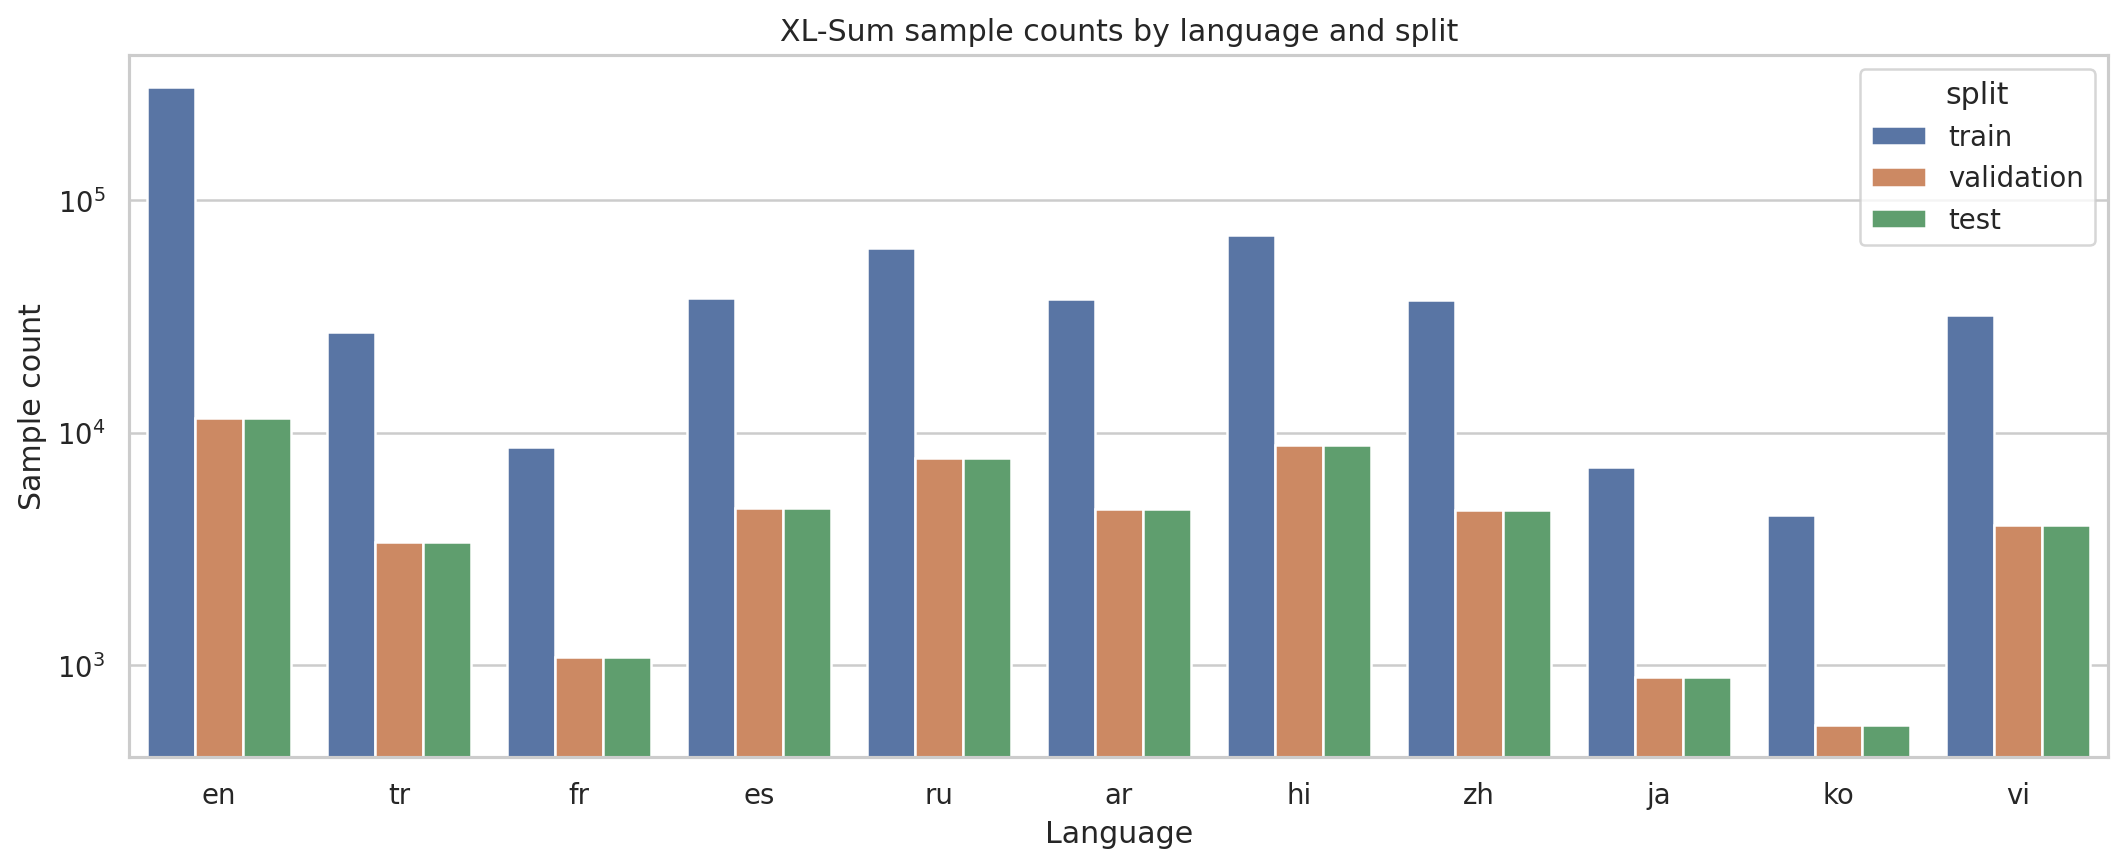
\includegraphics[width=.92\linewidth]{figures/sample_counts_by_language_split.png}
\caption{Nombre d'exemples XL-Sum par langue et par split}
\label{fig:xlsum-sample-counts}
\end{figure}

\subsection{Repartition linguistique}

La distribution par langue est desequilibree. L'anglais represente presque la moitie du split d'entrainement, alors que le coreen et le japonais sont beaucoup moins representes. Ce desequilibre a motive l'utilisation d'un lissage par langue dans la deuxieme chaine d'entrainement mBART.

\begin{table}[t]
\caption{Nombre d'exemples XL-Sum par langue}
\label{tab:xlsum-language-counts}
\centering
\begin{tabular}{|l|r|r|r|}
\hline
\textbf{Langue} & \textbf{Train} & \textbf{Validation} & \textbf{Test} \\
\hline
Anglais & 306522 & 11535 & 11535 \\
\hline
Turc & 27176 & 3397 & 3397 \\
\hline
Francais & 8697 & 1086 & 1086 \\
\hline
Espagnol & 38110 & 4763 & 4763 \\
\hline
Russe & 62243 & 7780 & 7780 \\
\hline
Arabe & 37519 & 4689 & 4689 \\
\hline
Hindi & 70778 & 8847 & 8847 \\
\hline
Chinois simplifie & 37362 & 4670 & 4670 \\
\hline
Japonais & 7113 & 889 & 889 \\
\hline
Coreen & 4407 & 550 & 550 \\
\hline
Vietnamien & 32111 & 4013 & 4013 \\
\hline
\end{tabular}
\end{table}

L'analyse du corpus montre aussi un comportement plutot abstractive. Sur les echantillons analyses, la nouveaute moyenne des bigrammes est d'environ 0.666 sur le train, 0.657 sur la validation et 0.658 sur le test. Cela signifie qu'une grande partie des bigrammes des resumes de reference n'apparait pas telle quelle dans l'article source. Les modeles doivent donc apprendre a reformuler, pas seulement a extraire des segments du texte.

\begin{figure}[t]
\centering
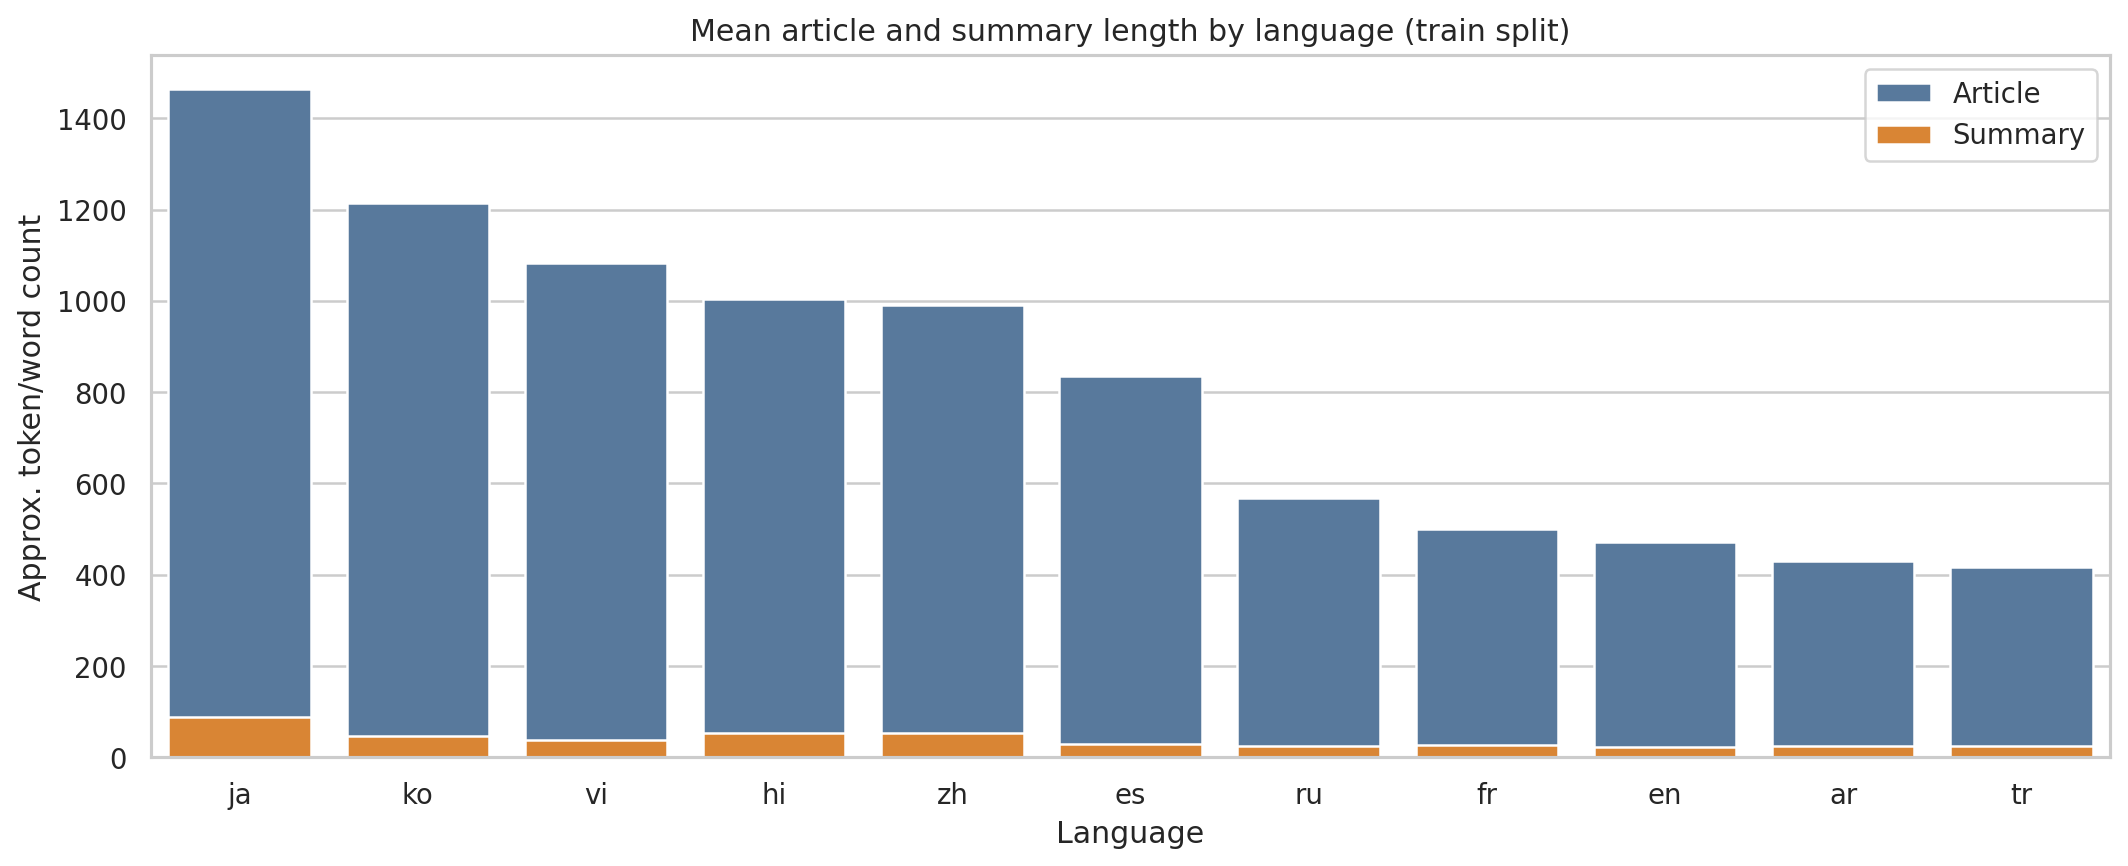
\includegraphics[width=.92\linewidth]{figures/mean_article_summary_length_train.png}
\caption{Longueur moyenne des articles et des resumes dans le split train}
\label{fig:xlsum-mean-length-train}
\end{figure}

\begin{figure}[t]
\centering
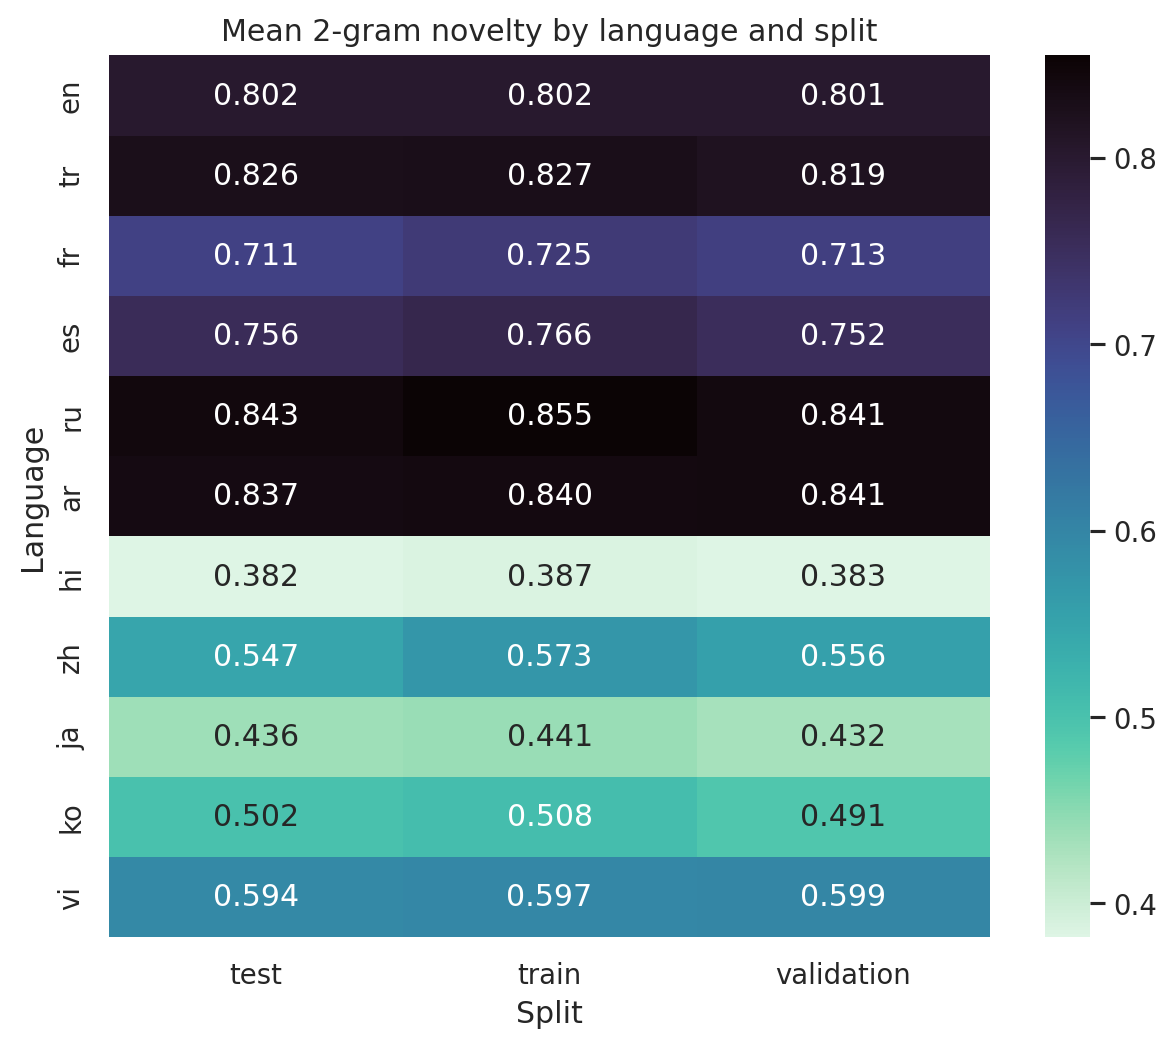
\includegraphics[width=.92\linewidth]{figures/novelty_2gram_heatmap.png}
\caption{Nouveaute moyenne des bigrammes par langue et par split}
\label{fig:xlsum-novelty-2gram}
\end{figure}

\section{Modeles integres dans le projet}

\subsection{Modeles disponibles dans le repertoire}

Le dossier \texttt{models/} contient six modeles de generation de resumes ou de traduction. Les modeles \texttt{bart\_large\_cnn}, \texttt{bart\_base\_cnn} et \texttt{bart\_reuters} sont des modeles BART destines principalement a l'anglais. Les modeles \texttt{mbart50\_xlsum} et \texttt{mbart-xlsum-2} sont les deux modeles multilingues entraines dans le cadre du projet. Le modele \texttt{mt5-xlsum} est un modele mT5 deja entraine, utilise comme reference comparative. Le dossier \texttt{mbart-large-50-many-to-many-mmt} sert a la traduction optionnelle des titres et resumes lorsque cette couche est activee.

\begin{table}[t]
\caption{Informations de configuration des principaux modeles}
\label{tab:model-configs}
\centering
\begin{tabular}{|p{3.1cm}|p{2.5cm}|r|r|r|r|}
\hline
\textbf{Modele} & \textbf{Famille} & \textbf{$d$} & \textbf{Enc.} & \textbf{Dec.} & \textbf{Vocab.} \\
\hline
\texttt{bart\_large\_cnn} & BART-large & 1024 & 12 & 12 & 50265 \\
\hline
\texttt{bart\_base\_cnn} & BART-base & 768 & 6 & 6 & 50265 \\
\hline
\texttt{bart\_reuters} & BART-base & 768 & 6 & 6 & 50265 \\
\hline
\texttt{mbart50\_xlsum} & mBART-50 & 1024 & 12 & 12 & 250054 \\
\hline
\texttt{mbart-xlsum-2} & mBART-50 & 1024 & 12 & 12 & 250054 \\
\hline
\texttt{mt5-xlsum} & mT5 & 768 & 12 & 12 & 250112 \\
\hline
\end{tabular}
\end{table}

Les deux modeles mBART ont la meme architecture sauvegardee: 12 couches encodeur, 12 couches decodeur, 16 tetes d'attention dans chaque bloc, dimension cachee 1024 et vocabulaire de 250.054 tokens. La difference entre ces deux modeles ne vient donc pas de l'architecture, mais des donnees d'entrainement, des hyperparametres, de la strategie de validation et du reechantillonnage linguistique.

\subsection{Entrainement des modeles mBART}

Le modele \texttt{mbart50\_xlsum} correspond a la premiere chaine d'entrainement. Il part de \texttt{facebook/mbart-large-50-many-to-many-mmt}, utilise \texttt{GEM/xlsum}, limite l'entree a 512 tokens et la cible a 96 tokens. L'entrainement est realise pendant 2 epochs avec un taux d'apprentissage de $3 \times 10^{-5}$. La taille de batch par appareil est 32 et l'accumulation de gradient est 8. L'evaluation generate est desactivee pendant l'entrainement et le meilleur checkpoint n'est pas selectionne automatiquement.

Le modele \texttt{mbart-xlsum-2} correspond a la chaine plus orientee qualite. Il part du meme modele de base, mais utilise \texttt{csebuetnlp/xlsum}. La longueur d'entree reste 512 tokens et la longueur cible passe a 64 tokens. L'entrainement est controle par \texttt{max\_steps=35000}, avec un taux d'apprentissage de $1 \times 10^{-4}$, \texttt{warmup\_steps=5000}, \texttt{adafactor}, \texttt{inverse\_sqrt}, une taille de batch par appareil de 8, une accumulation de gradient de 4 et une evaluation generate toutes les 5.000 etapes. Le meilleur checkpoint est charge a la fin selon \texttt{eval\_rougeL}.

\begin{table}[t]
\caption{Comparaison des deux chaines d'entrainement mBART}
\label{tab:mbart-training-numeric}
\centering
\begin{tabular}{|p{4.0cm}|p{4.4cm}|p{4.4cm}|}
\hline
\textbf{Element} & \textbf{\texttt{mbart50\_xlsum}} & \textbf{\texttt{mbart-xlsum-2}} \\
\hline
Modele de base & \texttt{facebook/mbart-large-50-many-to-many-mmt} & \texttt{facebook/mbart-large-50-many-to-many-mmt} \\
\hline
Jeu de donnees & \texttt{GEM/xlsum} & \texttt{csebuetnlp/xlsum} \\
\hline
Longueur source / cible & 512 / 96 tokens & 512 / 64 tokens \\
\hline
Duree & 2 epochs & 35.000 steps \\
\hline
Learning rate & $3 \times 10^{-5}$ & $1 \times 10^{-4}$ \\
\hline
Batch effectif & 32 $\times$ 8 & 8 $\times$ 4 \\
\hline
Optimisation & Parametres Trainer par defaut & \texttt{adafactor} + \texttt{inverse\_sqrt} \\
\hline
Validation & Desactivee pendant l'entrainement & Toutes les 5.000 etapes \\
\hline
Selection du checkpoint & Non & Oui, selon ROUGE-L \\
\hline
Equilibrage des langues & Melange standard & Lissage avec $\alpha=0.5$ \\
\hline
\end{tabular}
\end{table}

Le lissage linguistique utilise dans la deuxieme chaine diminue la domination des langues tres frequentes. Si $n_l$ est le nombre d'exemples d'une langue $l$ et $L$ l'ensemble des langues, la probabilite de reechantillonnage est:

\begin{equation}
p_l = \frac{n_l^{\alpha}}{\sum_{j \in L} n_j^{\alpha}},
\quad \alpha = 0.5.
\label{eq:application-language-smoothing}
\end{equation}

Avec $\alpha=1$, la distribution suit directement les tailles originales des langues. Avec $\alpha=0.5$, les grandes langues restent importantes, mais les langues plus petites deviennent plus visibles pendant l'entrainement.

\section{Architecture de l'application}

\subsection{Flux de traitement}

L'application web se trouve dans le dossier \texttt{app/}. Elle expose une interface et une API permettant de consulter des actualites resumees. Le systeme ne genere pas les resumes au moment exact de chaque requete utilisateur. La generation est deplacee dans un processus d'ingestion en arriere-plan. Cette architecture reduit la latence percue par l'utilisateur et permet de stocker plusieurs resumes par article et par modele.

Le flux numerique est le suivant. Le scheduler lance periodiquement l'ingestion. Le service de nouvelles collecte les entrees RSS selon les filtres de langue, source, sujet, pays et region. Le service d'article tente d'ouvrir le lien original, d'extraire le corps de l'article et de nettoyer le texte. Le service de resume appelle le modele choisi, applique un post-traitement, puis utilise un resume extractif de secours si la sortie est vide ou degeneree. Enfin, le service de stockage ecrit les articles et les resumes dans SQLite.

\subsection{Parametres applicatifs}

Les parametres principaux de l'application sont definis dans \texttt{app/core.py} et dans les variables d'environnement. Par defaut, le modele principal est \texttt{mbart50\_xlsum}. La limite de texte envoyee au modele est \texttt{MAX\_INPUT\_CHARS=3500}. La tokenisation limite l'entree a 1024 tokens. Le nombre maximum de tokens de resume par defaut est \texttt{SUMMARY\_MAX\_TOKENS=96}.

Pour les modeles mBART, l'application configure le code de langue mBART associe a la langue source, puis force le token de debut de generation correspondant. Les parametres de generation mBART par defaut sont: longueur maximale 90, longueur minimale 24, 5 beams et penalite de longueur 1.1. Pour le turc, le systeme utilise un reglage specifique: longueur maximale 84, longueur minimale 26, 6 beams, \texttt{no\_repeat\_ngram\_size=4} et penalite de repetition 1.2. Pour \texttt{mt5-xlsum}, la longueur maximale est 84, la longueur minimale 20 et le nombre de beams 4.

La base SQLite contient trois tables principales. \texttt{news\_items} stocke les articles, les metadonnees, la langue, la source et le texte extrait. \texttt{news\_summaries} stocke le resume produit pour un couple article-modele-langue, avec une contrainte d'unicite sur \texttt{news\_item\_id}, \texttt{model\_key} et \texttt{language\_key}. \texttt{ingest\_runs} garde l'historique des executions d'ingestion, leur configuration, leurs statistiques et les erreurs eventuelles.

\section{Pipeline d'evaluation}

\subsection{Configuration experimentale}

L'evaluation finale est produite par le notebook \texttt{evaluation/pipelines/xlsum\_model\_evaluation\_pipeline\_full.ipynb}. La configuration sauvegardee dans \texttt{evaluation/xlsum\_eval\_full/run\_config.json} indique que le split utilise est \texttt{test}, que les titres ne sont pas ajoutes a l'entree du modele, que la taille de batch est 8, que l'entree est limitee a 512 tokens et que l'execution utilise CUDA avec FP16 lorsque c'est disponible.

Les modeles evalues dans le rapport final sont \texttt{mbart50\_xlsum}, \texttt{mbart-xlsum-2} et \texttt{mt5-xlsum}. Les modeles BART anglais sont definis dans la pipeline, mais le rapport numerique final se concentre sur les modeles multilingues, car le scenario principal du projet est le resume d'actualites dans plusieurs langues.

La pipeline bloque explicitement l'utilisation du split \texttt{train} pour eviter une fuite de donnees. Elle produit notamment \texttt{detailed\_metrics.csv}, \texttt{detailed\_predictions.jsonl}, \texttt{model\_language\_summary.csv}, \texttt{model\_overall\_macro\_summary.csv}, \texttt{xlsum\_evaluation\_report.xlsx}, \texttt{report.md} et plusieurs figures.

\subsection{Formules des metriques classiques}

Soit $r$ le resume de reference et $\hat{y}$ le resume genere. Pour ROUGE-$N$, on note $G_N(x)$ le multiensemble des $N$-grammes du texte $x$. La precision, le rappel et la F-mesure sont:

\begin{align}
P_N &= \frac{|G_N(\hat{y}) \cap G_N(r)|}{|G_N(\hat{y})|}, \\
R_N &= \frac{|G_N(\hat{y}) \cap G_N(r)|}{|G_N(r)|}, \\
F_N &= \frac{2 P_N R_N}{P_N + R_N}.
\label{eq:rouge-n}
\end{align}

ROUGE-L remplace le recouvrement de $N$-grammes par la longueur de la plus longue sous-sequence commune, notee $\operatorname{LCS}(\hat{y}, r)$:

\begin{align}
P_L &= \frac{\operatorname{LCS}(\hat{y}, r)}{|\hat{y}|}, \\
R_L &= \frac{\operatorname{LCS}(\hat{y}, r)}{|r|}, \\
F_L &= \frac{2 P_L R_L}{P_L + R_L}.
\label{eq:rouge-l}
\end{align}

BLEU est calcule avec \texttt{sacrebleu} au niveau phrase, sans retokenisation supplementaire et avec lissage exponentiel. Sa forme generale est:

\begin{equation}
\operatorname{BLEU} = \operatorname{BP} \cdot
\exp\left(\sum_{n=1}^{4} w_n \log p_n\right),
\label{eq:bleu}
\end{equation}

ou $p_n$ represente la precision modifiee des $n$-grammes, $w_n$ les poids des ordres de $n$-grammes et $\operatorname{BP}$ la penalite de brievete.

La metrique \texttt{METEOR-lite} implementee dans la pipeline utilise les correspondances exactes de tokens. Si $m$ est le nombre de tokens apparies, $P_m=m/|\hat{y}|$ et $R_m=m/|r|$, alors:

\begin{align}
F_{\mathrm{meteor}} &= \frac{10 P_m R_m}{R_m + 9P_m}, \\
\operatorname{Penalty} &= 0.5 \left(\frac{\operatorname{chunks}}{m}\right)^3, \\
\operatorname{METEOR\mbox{-}lite} &= F_{\mathrm{meteor}}(1-\operatorname{Penalty}).
\label{eq:meteor-lite}
\end{align}

\subsection{Metriques source et comportement}

Les metriques classiques sont completees par des metriques liees a la source et au comportement de generation. La couverture source mesure la part du vocabulaire du resume qui est presente dans l'article source:

\begin{equation}
S_{\mathrm{cov}} =
\frac{|V(\hat{y}) \cap V(x)|}{|V(\hat{y})|}.
\label{eq:source-coverage}
\end{equation}

Le rappel source mesure la part du vocabulaire de l'article qui est reprise dans le resume:

\begin{equation}
S_{\mathrm{rec}} =
\frac{|V(\hat{y}) \cap V(x)|}{|V(x)|}.
\label{eq:source-recall}
\end{equation}

Le taux de compression utilise dans l'evaluation est le rapport entre la longueur source et la longueur generee:

\begin{equation}
\operatorname{compression} = \frac{|x|}{|\hat{y}|}.
\label{eq:compression-ratio}
\end{equation}

La latence est aussi normalisee par 1.000 tokens source:

\begin{equation}
\operatorname{latency}_{1k} =
\frac{\operatorname{latency}_{sec}}{\max(|x|/1000, 10^{-6})}.
\label{eq:latency-1k}
\end{equation}

La repetition est mesuree par le taux de $n$-grammes repetes dans le resume genere. Dans la pipeline, la valeur utilisee dans les scores composites est surtout \texttt{repetition\_3gram}:

\begin{equation}
\operatorname{rep}_{n} =
1 - \frac{|\operatorname{unique}(G_n(\hat{y}))|}{|G_n(\hat{y})|}.
\label{eq:repetition-ngram}
\end{equation}

La nouveaute mesure la part des $n$-grammes du resume qui ne sont pas presents dans l'article source. Elle sert a observer le degre d'abstraction du resume:

\begin{equation}
\operatorname{novelty}_{n} =
1 - \frac{|\{g \in G_n(\hat{y}) : g \in G_n(x)\}|}{|G_n(\hat{y})|}.
\label{eq:novelty-ngram}
\end{equation}

Les fragments extractifs sont les sequences de tokens du resume qui apparaissent aussi dans la source. Si $F$ est l'ensemble des longueurs de fragments trouves par l'algorithme de correspondance et si $l_f$ est la longueur du fragment $f$, alors:

\begin{align}
F_{\mathrm{cov}} &= \frac{\sum_{f \in F} l_f}{|\hat{y}|}, \\
F_{\mathrm{dens}} &= \frac{\sum_{f \in F} l_f^2}{|\hat{y}|}.
\label{eq:fragment-coverage-density}
\end{align}

La composante de lisibilite depend de la langue. Pour l'anglais, la pipeline utilise le score de Flesch, normalise dans $[0,1]$:

\begin{equation}
R_{\mathrm{read}} =
\operatorname{clip}_{[0,1]}\left(\frac{\operatorname{Flesch}(\hat{y}) + 20}{120}\right).
\label{eq:readability-component-en}
\end{equation}

Pour les autres langues, la pipeline utilise un score heuristique de longueur moyenne de phrase. Si $\bar{s}$ est la longueur moyenne des phrases, l'intervalle ideal est $[12,45]$ pour le chinois, le japonais et le coreen, et $[8,25]$ pour les autres langues:

\begin{equation}
I_{\mathrm{sent}} =
\begin{cases}
0, & \bar{s} \leq 0, \\
\operatorname{clip}_{[0,1]}(\bar{s}/a), & 0 < \bar{s} < a, \\
1, & a \leq \bar{s} \leq b, \\
\operatorname{clip}_{[0,1]}(1-(\bar{s}-b)/b), & \bar{s} > b.
\end{cases}
\label{eq:ideal-sentence-length}
\end{equation}

Dans cette formule, $(a,b)=(12,45)$ pour les langues CJK et $(a,b)=(8,25)$ pour les autres langues. Pour les langues non anglaises, $R_{\mathrm{read}}$ est remplace par $I_{\mathrm{sent}}$.

\subsection{Scores proxy composites}

Les scores proxy composites sont bornes dans l'intervalle $[0,1]$ avec l'operateur $\operatorname{clip}_{[0,1]}$. Les poids ont ete choisis de maniere heuristique selon une logique de signal principal et de correction secondaire: le signal le plus directement lie a la dimension mesuree recoit le poids dominant, tandis que les autres signaux corrigent les cas limites. Ces scores ne sont donc pas des metriques humaines apprises, mais des indicateurs automatiques reproductibles pour comparer les modeles dans les memes conditions.

La coherence combine la stabilite des longueurs de phrases, le faible taux de repetition et une longueur de phrase ideale. Le poids principal est donne a la regularite des longueurs de phrases, car elle mesure directement la stabilite structurelle du resume:

\begin{align}
C_{\mathrm{coh}} = \operatorname{clip}_{[0,1]}(&0.50 \cdot \operatorname{clip}_{[0,1]}(1-\sigma_{\mathrm{sent}}/20) \nonumber\\
&+0.30 \cdot (1-\operatorname{rep}_{3g}) \nonumber\\
&+0.20 \cdot I_{\mathrm{sent}}).
\label{eq:coherence}
\end{align}

L'exactitude combine l'accord avec la reference et la couverture de la source. Le poids 0.70 est donne a l'accord avec le resume humain, car la reference reste le signal principal de correction; le poids 0.30 ajoute une contrainte de rattachement au texte source:

\begin{align}
A_{\mathrm{ref}} &= \operatorname{mean}(\operatorname{ROUGE\mbox{-}L}, \operatorname{BLEU}, \operatorname{METEOR\mbox{-}lite}), \\
C_{\mathrm{acc}} &= \operatorname{clip}_{[0,1]}(0.70 \cdot A_{\mathrm{ref}} + 0.30 \cdot S_{\mathrm{cov}}).
\label{eq:accuracy}
\end{align}

La clarte combine la lisibilite et l'absence de repetition. La lisibilite recoit le poids dominant, car elle mesure directement la facilite de lecture, tandis que la repetition corrige les sorties artificiellement lisibles mais redondantes:

\begin{equation}
C_{\mathrm{clar}} =
\operatorname{clip}_{[0,1]}(0.70 \cdot R_{\mathrm{read}} + 0.30 \cdot (1-\operatorname{rep}_{3g})).
\label{eq:clarity}
\end{equation}

La pertinence combine le rappel ROUGE-1 et le rappel source. Le rappel ROUGE-1 est dominant parce qu'il mesure la couverture du contenu attendu dans la reference; le rappel source ajoute une indication de couverture du document original:

\begin{equation}
C_{\mathrm{rel}} =
\operatorname{clip}_{[0,1]}(0.70 \cdot R_{1} + 0.30 \cdot S_{\mathrm{rec}}).
\label{eq:relevance}
\end{equation}

L'efficacite combine la vitesse et la compression. La vitesse normalisee recoit le poids 0.60, car l'application vise un usage interactif; la compression recoit le poids 0.40, car un resume rapide mais trop long serait peu utile:

\begin{align}
L_{\mathrm{score}} &= \frac{1}{1+\operatorname{latency}_{1k}}, \\
K_{\mathrm{score}} &= \operatorname{clip}_{[0,1]}\left(\frac{\operatorname{compression}-2}{18}\right), \\
C_{\mathrm{eff}} &= \operatorname{clip}_{[0,1]}(0.60 \cdot L_{\mathrm{score}} + 0.40 \cdot K_{\mathrm{score}}).
\label{eq:efficiency}
\end{align}

Le score global de capacite est la moyenne de ces cinq dimensions:

\begin{equation}
C_{\mathrm{all}} =
\operatorname{mean}(C_{\mathrm{coh}}, C_{\mathrm{acc}}, C_{\mathrm{clar}}, C_{\mathrm{rel}}, C_{\mathrm{eff}}).
\label{eq:capability-overall-application}
\end{equation}

Deux scores de qualite supplementaires sont utilises. La fidelite a la source combine la couverture source et la couverture des fragments extraits. La couverture source recoit le poids principal parce qu'elle penalise les mots absents de l'article, tandis que les fragments extraits renforcent l'indication de rattachement direct au texte:

\begin{equation}
Q_{\mathrm{fact}} =
\operatorname{clip}_{[0,1]}(0.60 \cdot S_{\mathrm{cov}} + 0.40 \cdot F_{\mathrm{cov}}).
\label{eq:factuality}
\end{equation}

La completude combine le rappel ROUGE-1 et l'alignement de longueur avec le resume de reference. Le rappel ROUGE-1 mesure la presence du contenu attendu; l'alignement de longueur evite de favoriser des resumes trop courts ou trop longs:

\begin{align}
A_{\mathrm{len}} &=
\operatorname{clip}_{[0,1]}\left(1-\frac{\left||\hat{y}|-|r|\right|}{\max(|r|,1)}\right), \\
Q_{\mathrm{comp}} &=
\operatorname{clip}_{[0,1]}(0.70 \cdot R_1 + 0.30 \cdot A_{\mathrm{len}}).
\label{eq:completeness}
\end{align}
